\setcounter{section}{5}
\setcounter{subsection}{0}
\subsection{TCP- und UDP-Ports in Wireshark}

\begin{enumerate}[(a)]
    \item Finden Sie den Destination-Port der Segmente. Welche Protokolle der
        Anwendungsschicht verbergen sich dahinter?

        \begin{table}[h]
            \centering
            \begin{tabular}{c|c|c}
                Port & Protokoll & Wireshark-Mitschnitt \\
                \hline
                21   & FTP       & \ref{fig:5.1.a.ftp} \\
                22   & SSH       & \ref{fig:5.1.a.ssh} \\
                23   & TELNET    & \ref{fig:5.1.a.telnet} \\
                53   & DNS       & \ref{fig:5.1.a.dns} \\
                80   & HTTP      & \ref{fig:5.1.a.http} \\
                443  & HTTPS     & \ref{fig:5.1.a.https}
            \end{tabular}
        \end{table}

    \item Wie lang sind die kürzesten bzw. längsten Segmente?

        66 und 9750. Siehe Abbildungen~\ref{fig:5.1.b.1}~und~\ref{fig:5.1.b.2}

    \item Erstellen Sie eine Statistik aller verwendeten Anwendungsprotokolle
        und der damit ausgetauschten Datenmengen.

        Siehe Abbildung~\ref{fig:5.1.c}

    \item Sowohl UDP als auch TCP verwenden Port-Nummern, um das Ziel bei der
        Zustellung einer Nachricht anzugeben. Geben Sie Gründe an, warum die
        beiden Protokolle Port-Nummer anstelle der Prozesskennung der
        Anwendungsschicht verwenden.

        \begin{itemize}
            \item PIDs sind betriebssystemabhängig, Port-Nummern nicht. 
            \item PIDs sind lokale Informationen, die nur auf dem eigenen
                Rechner Sinn ergeben.
            \item Port-Nummern sind global standardisiert (z.B. Port 80 für
                HTTP), was es Clients ermöglicht, Dienste unabhängig vom
                Betriebssystem anzusprechen.
        \end{itemize}
\end{enumerate}

\begin{figure}[p]
    \centering
    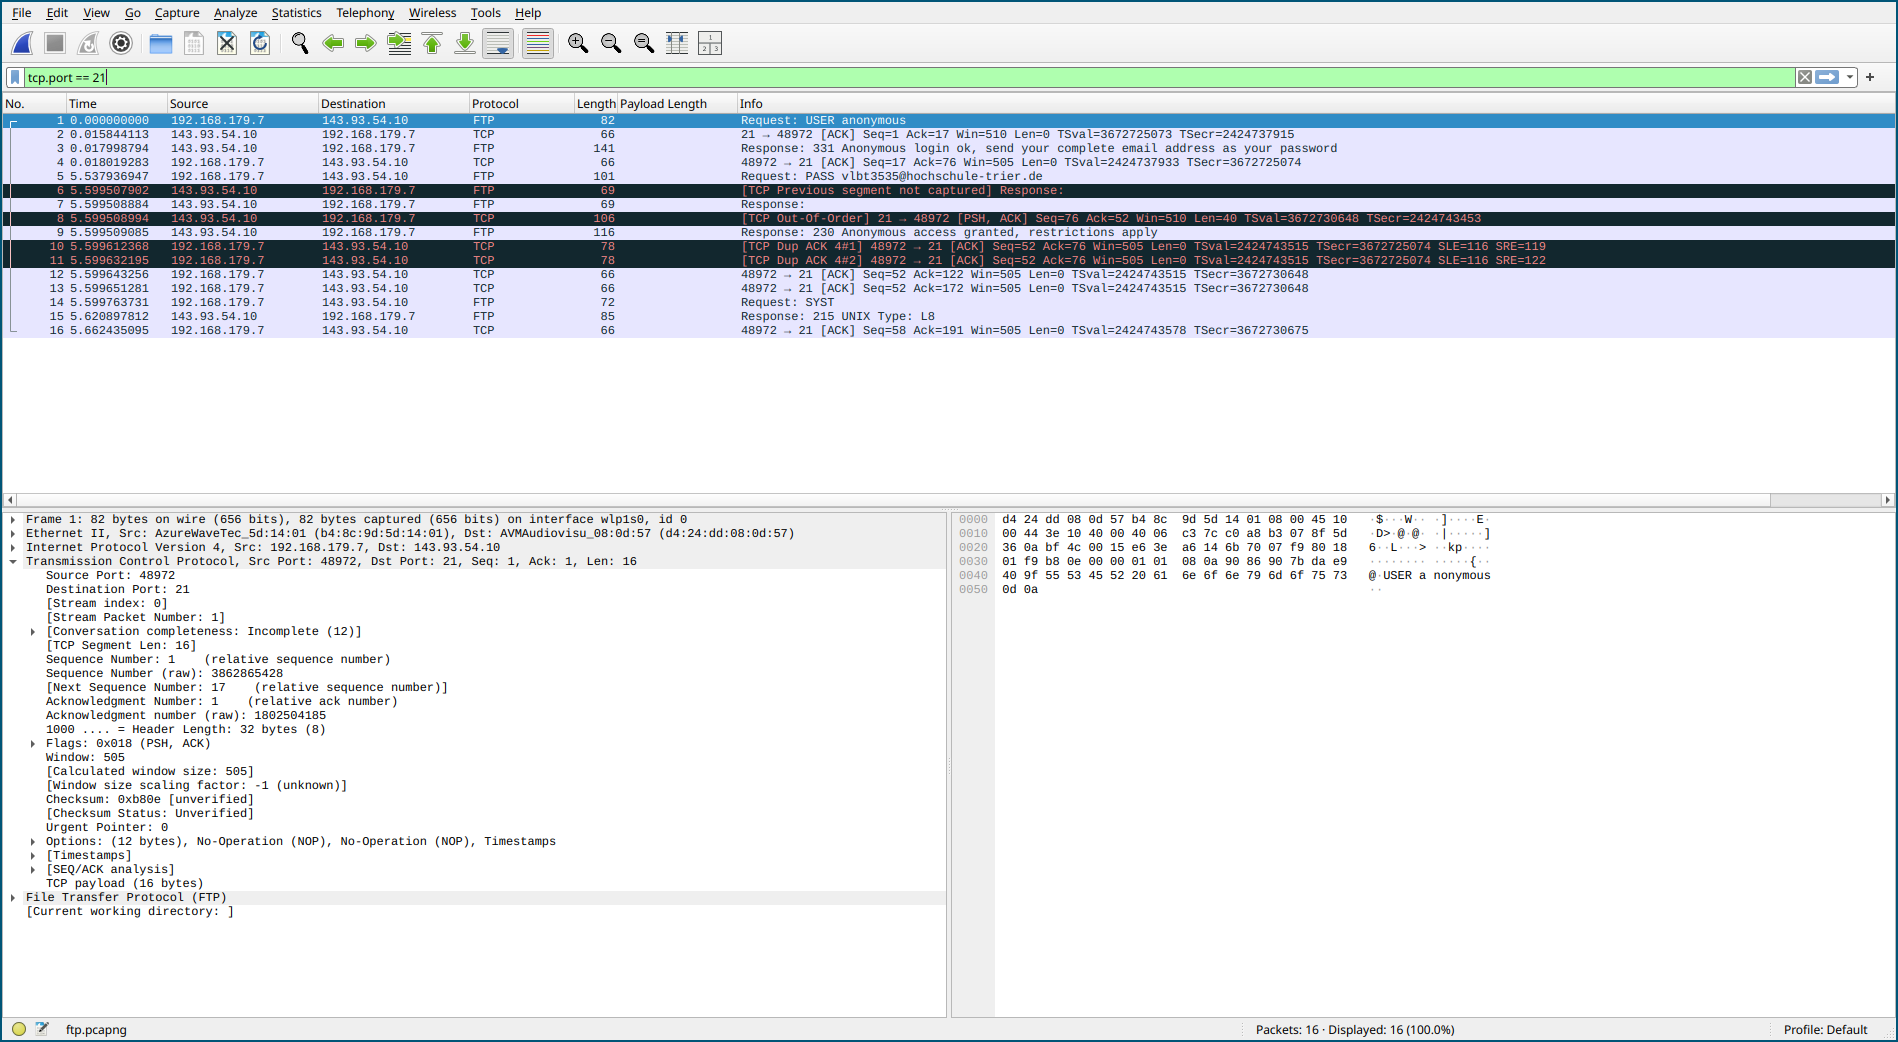
\includegraphics[width=1\textwidth]{./assets/5.1.a.ftp.png}
    \caption{FTP-Datenverkehr}
    \label{fig:5.1.a.ftp}
\end{figure}

\begin{figure}[p]
    \centering
    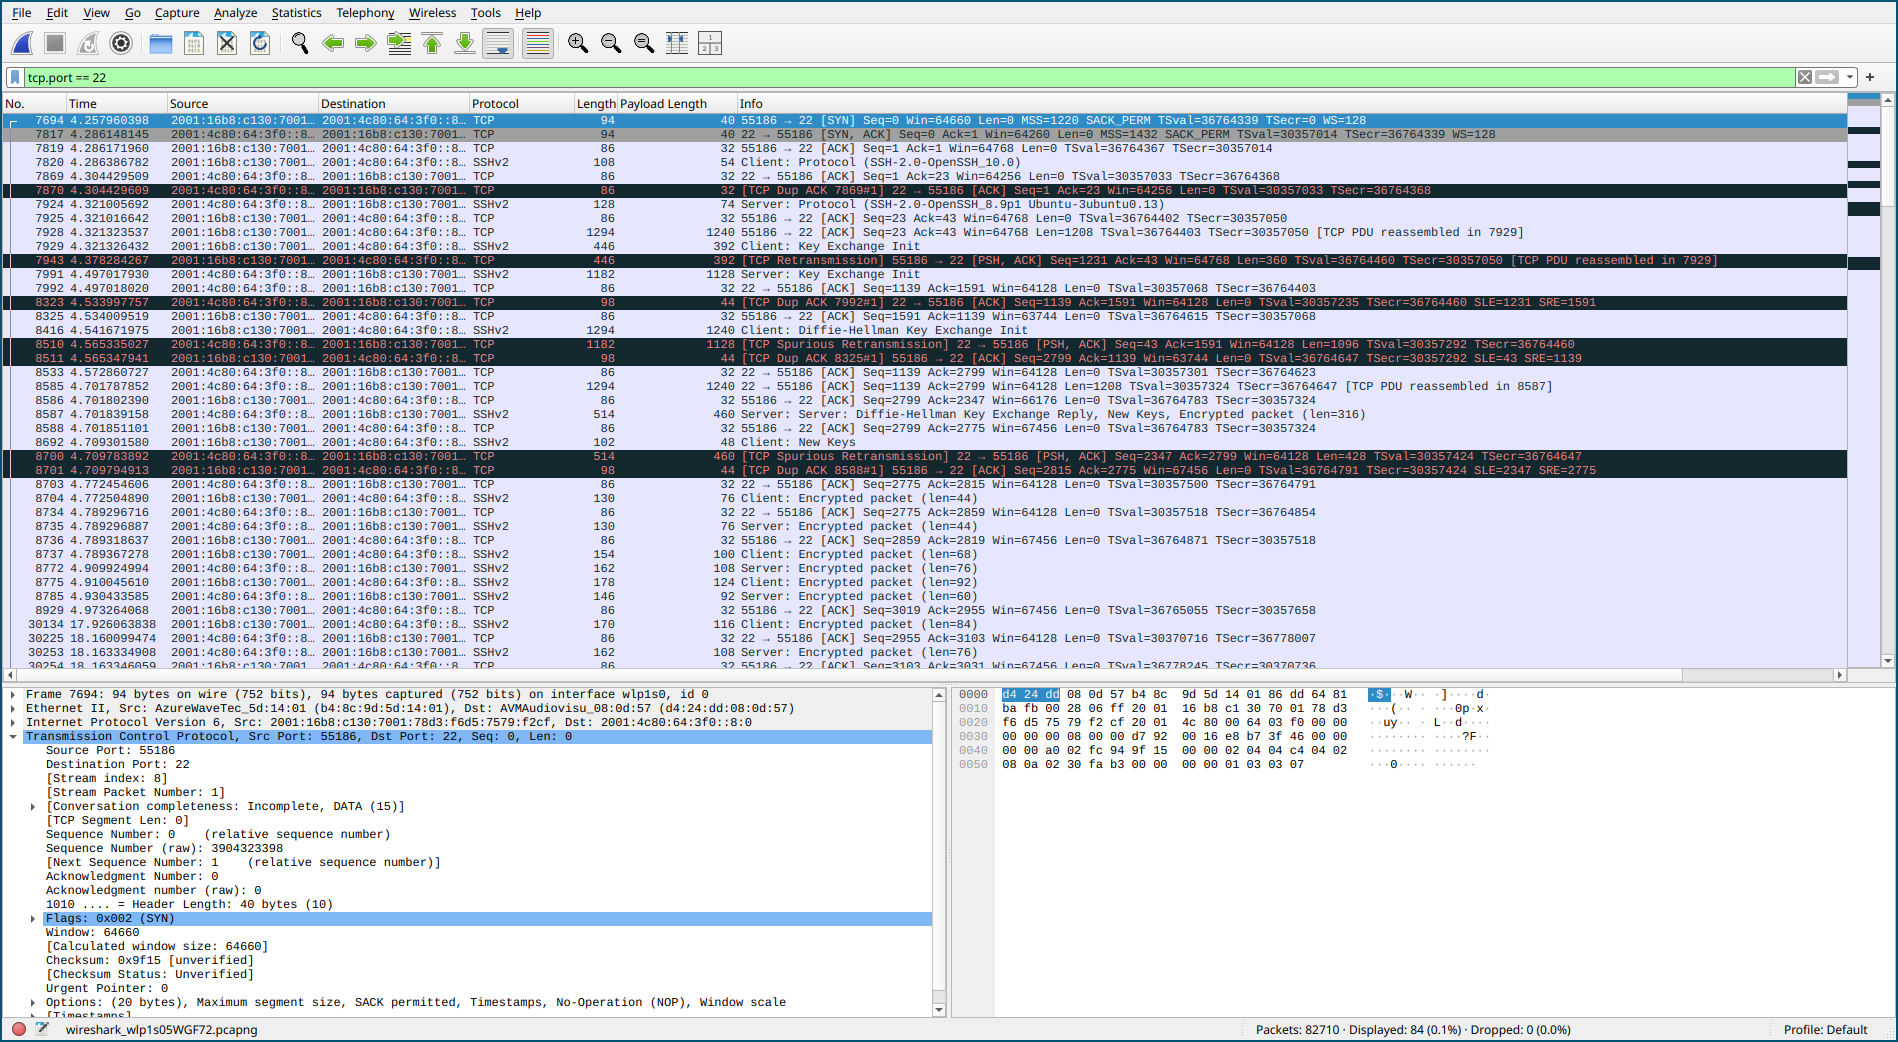
\includegraphics[width=1\textwidth]{./assets/5.1.a.ssh.png}
    \caption{SSH-Datenverkehr}
    \label{fig:5.1.a.ssh}
\end{figure}

\FloatBarrier

\begin{figure}[p]
    \centering
    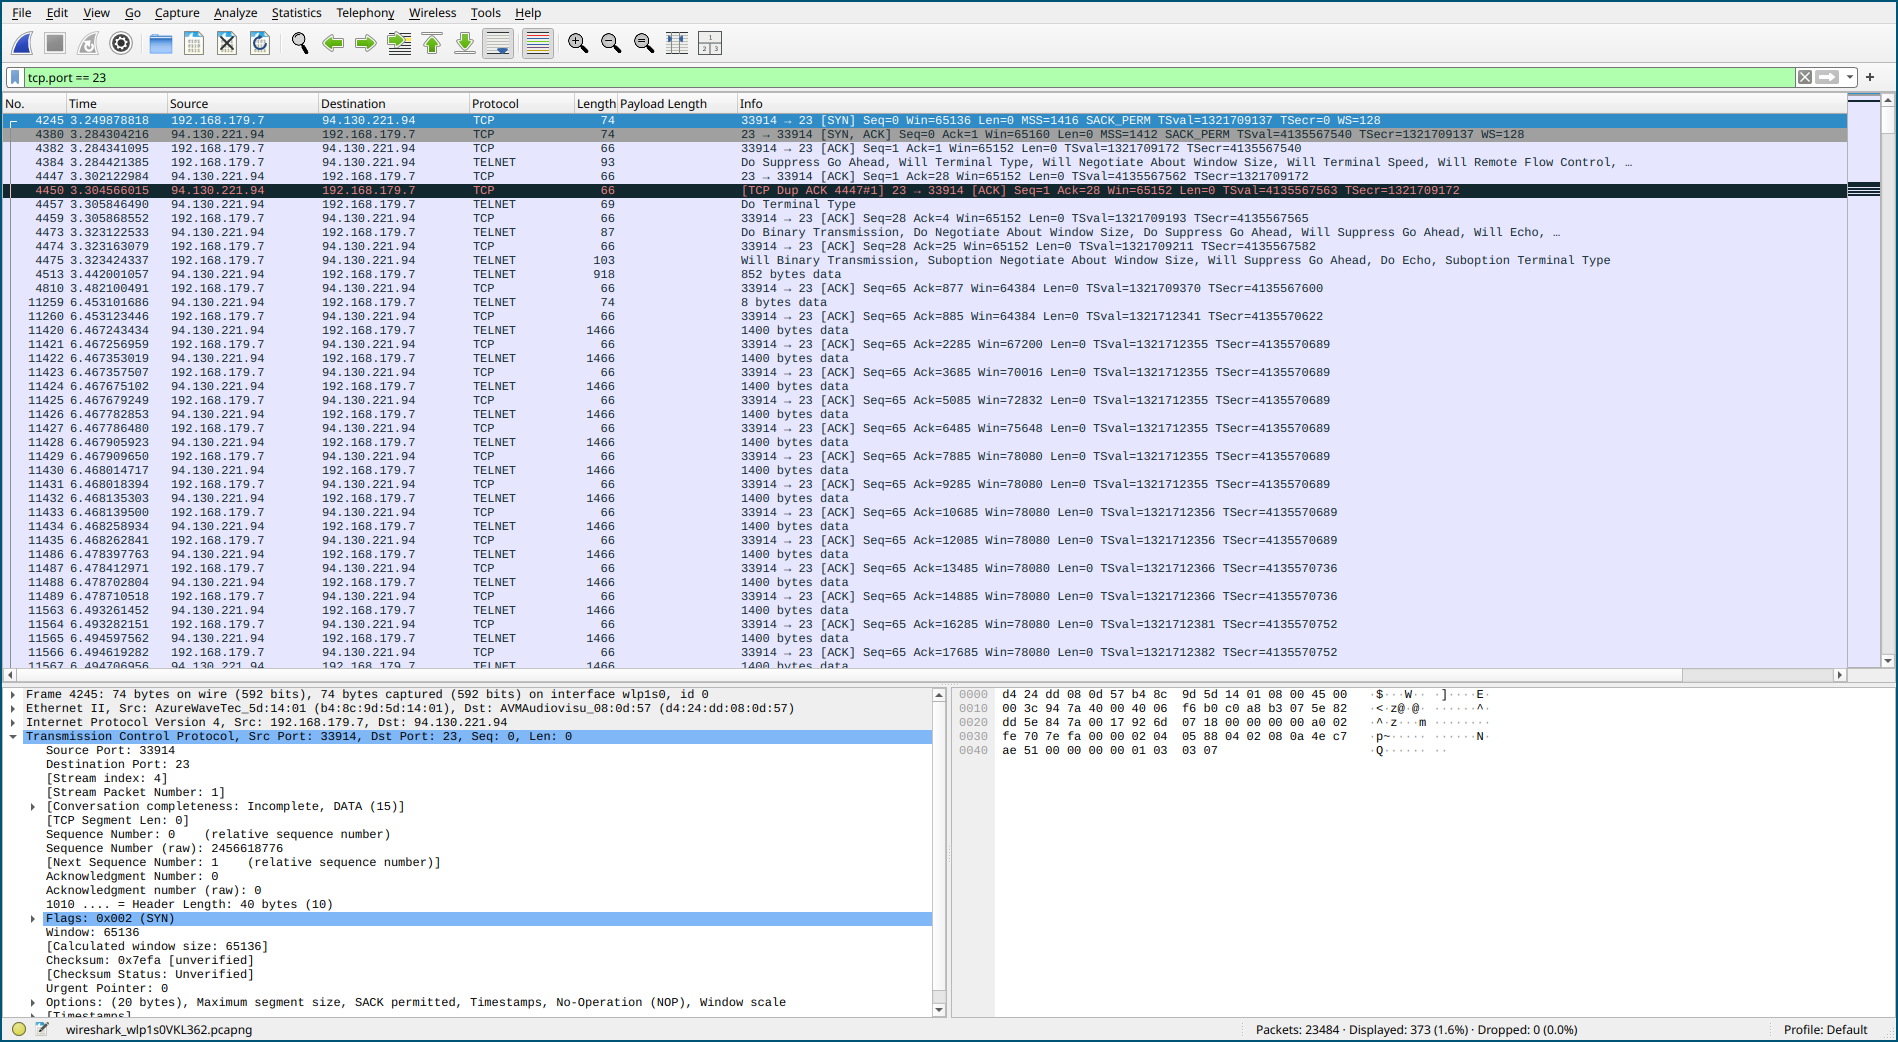
\includegraphics[width=1\textwidth]{./assets/5.1.a.telnet.png}
    \caption{TELNET-Datenverkehr}
    \label{fig:5.1.a.telnet}
\end{figure}

\begin{figure}[p]
    \centering
    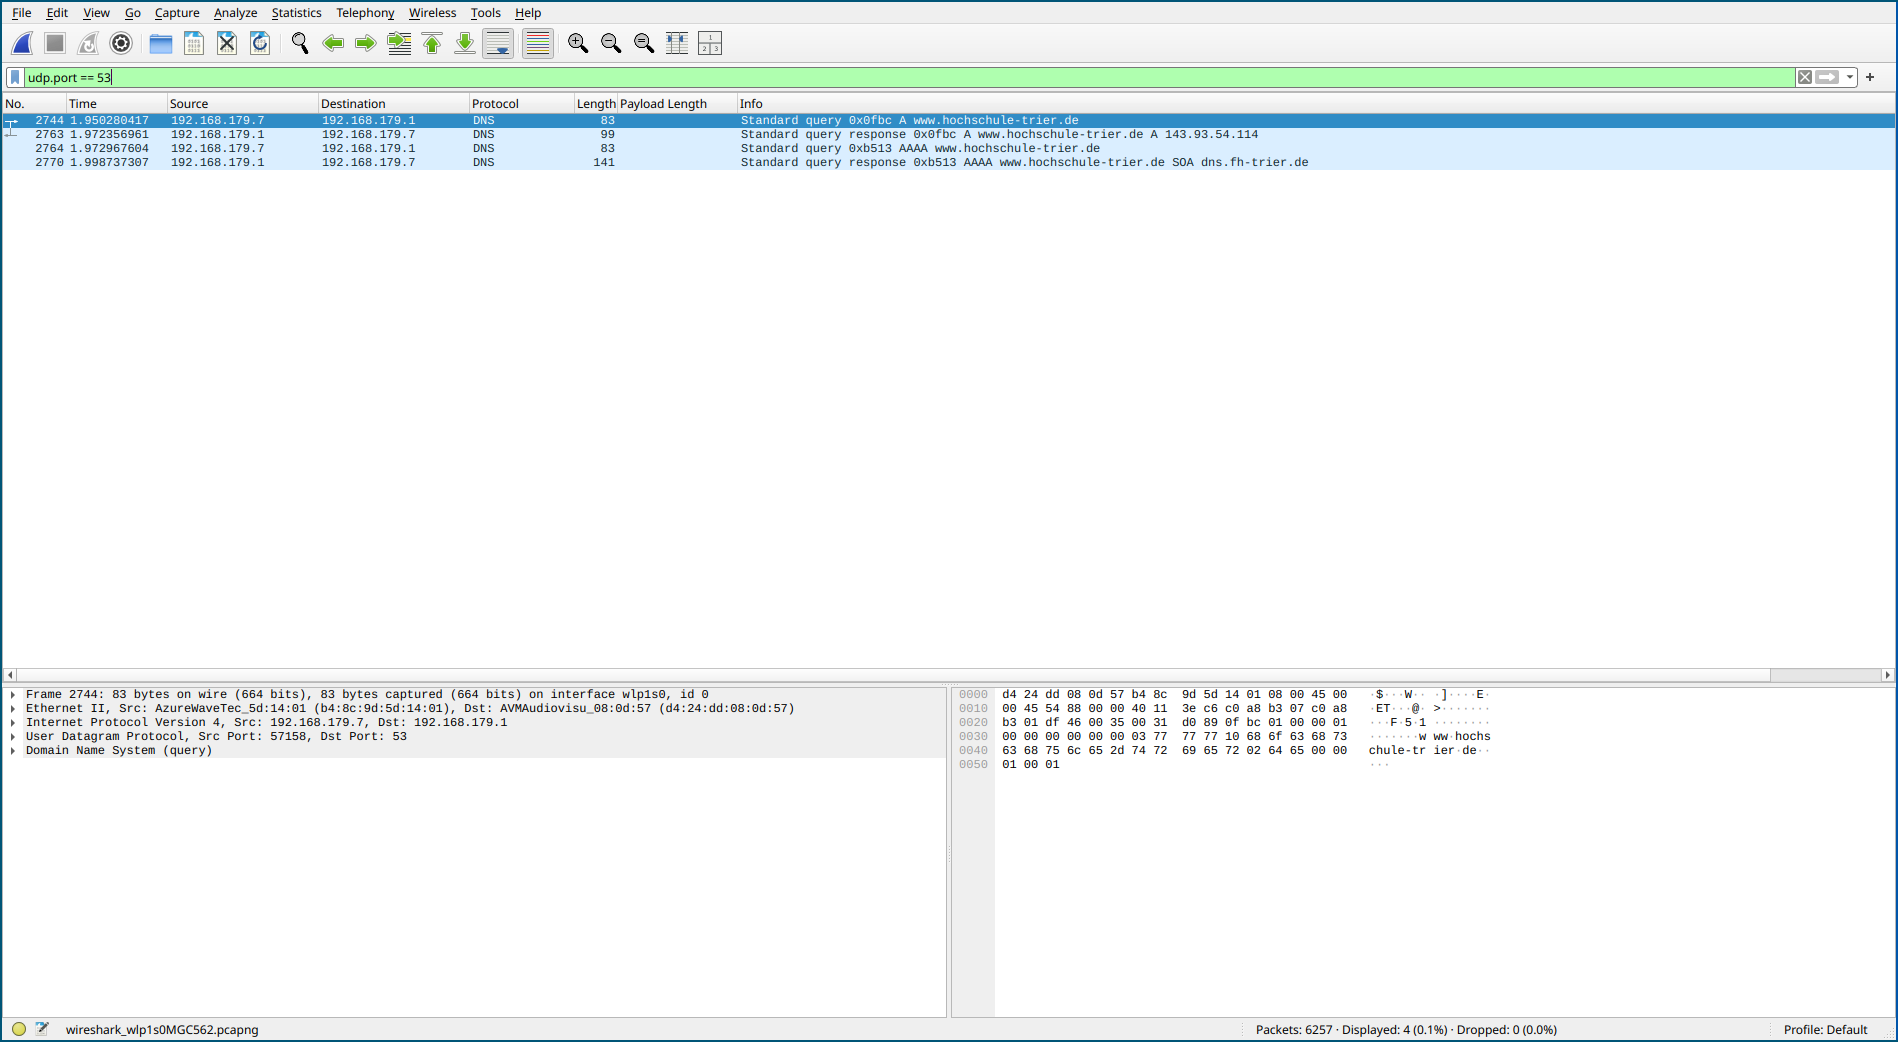
\includegraphics[width=1\textwidth]{./assets/5.1.a.dns.png}
    \caption{DNS-Datenverkehr}
    \label{fig:5.1.a.dns}
\end{figure}

\FloatBarrier

\begin{figure}[p]
    \centering
    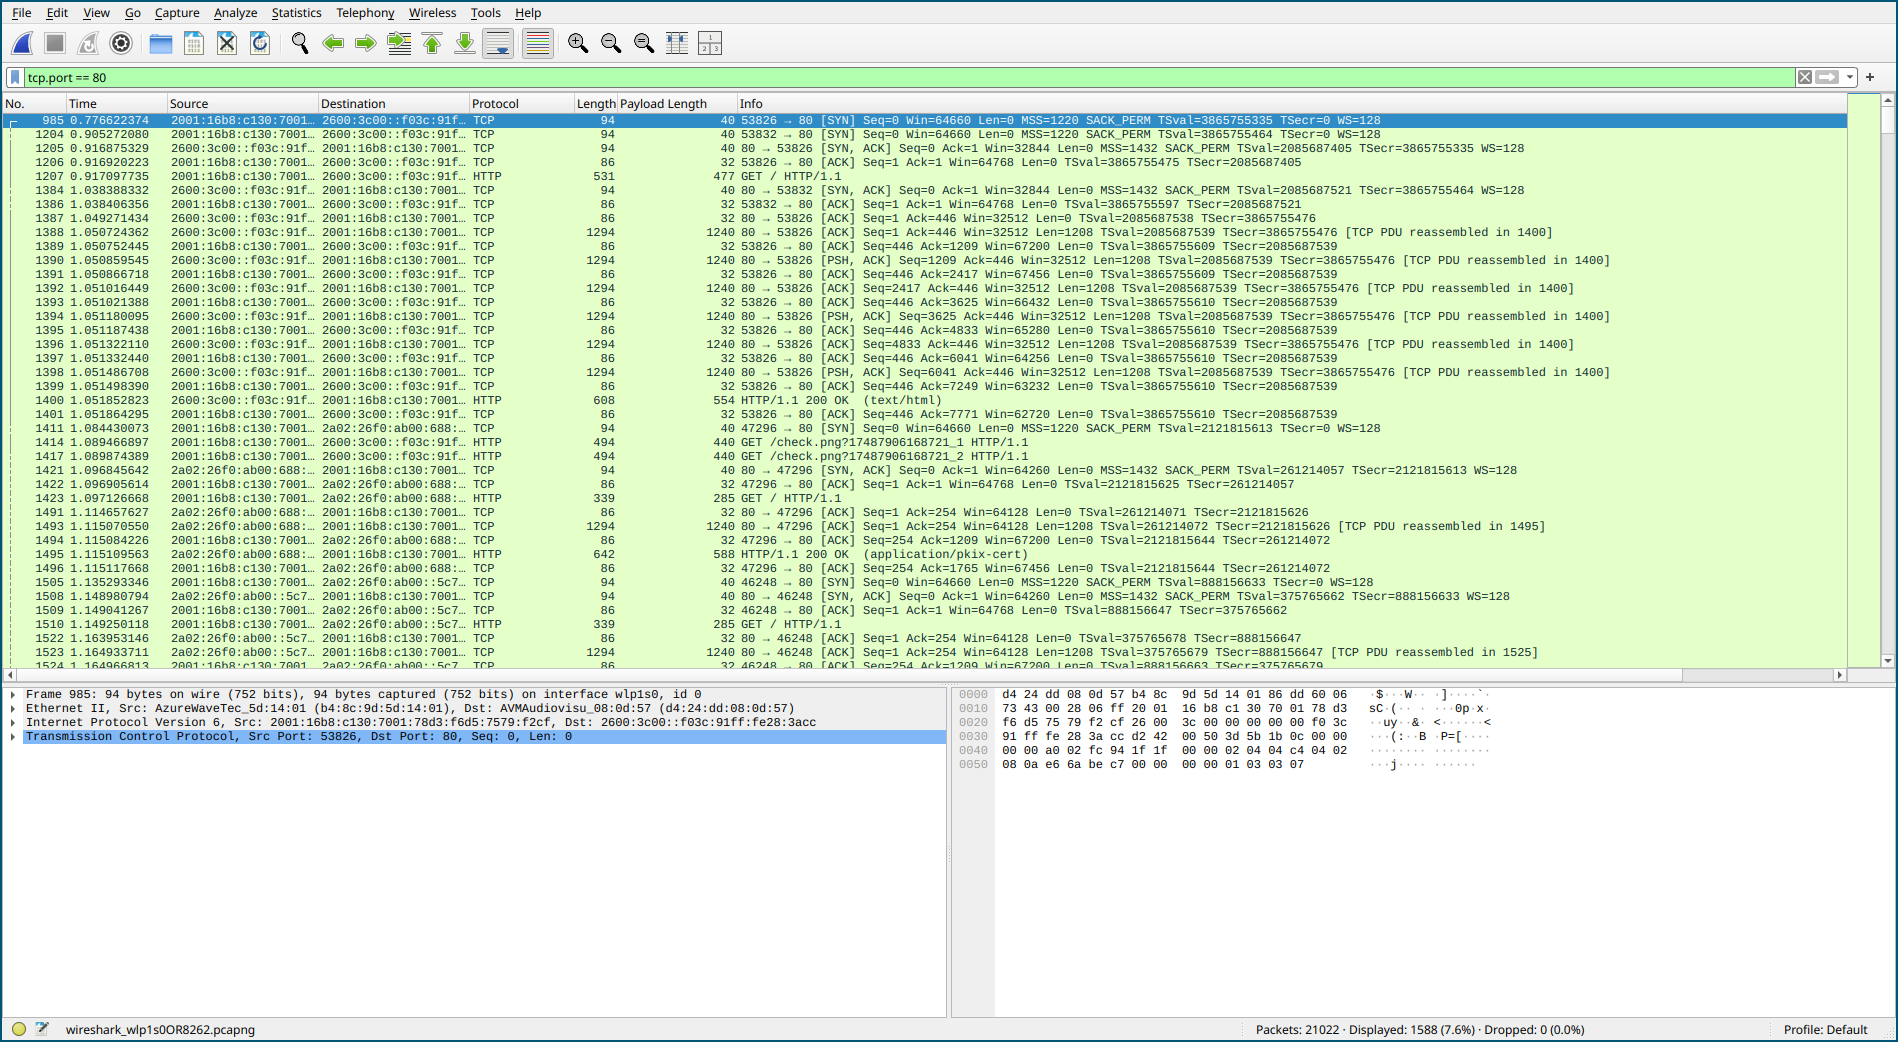
\includegraphics[width=1\textwidth]{./assets/5.1.a.http.png}
    \caption{HTTP-Datenverkehr}
    \label{fig:5.1.a.http}
\end{figure}

\begin{figure}[p]
    \centering
    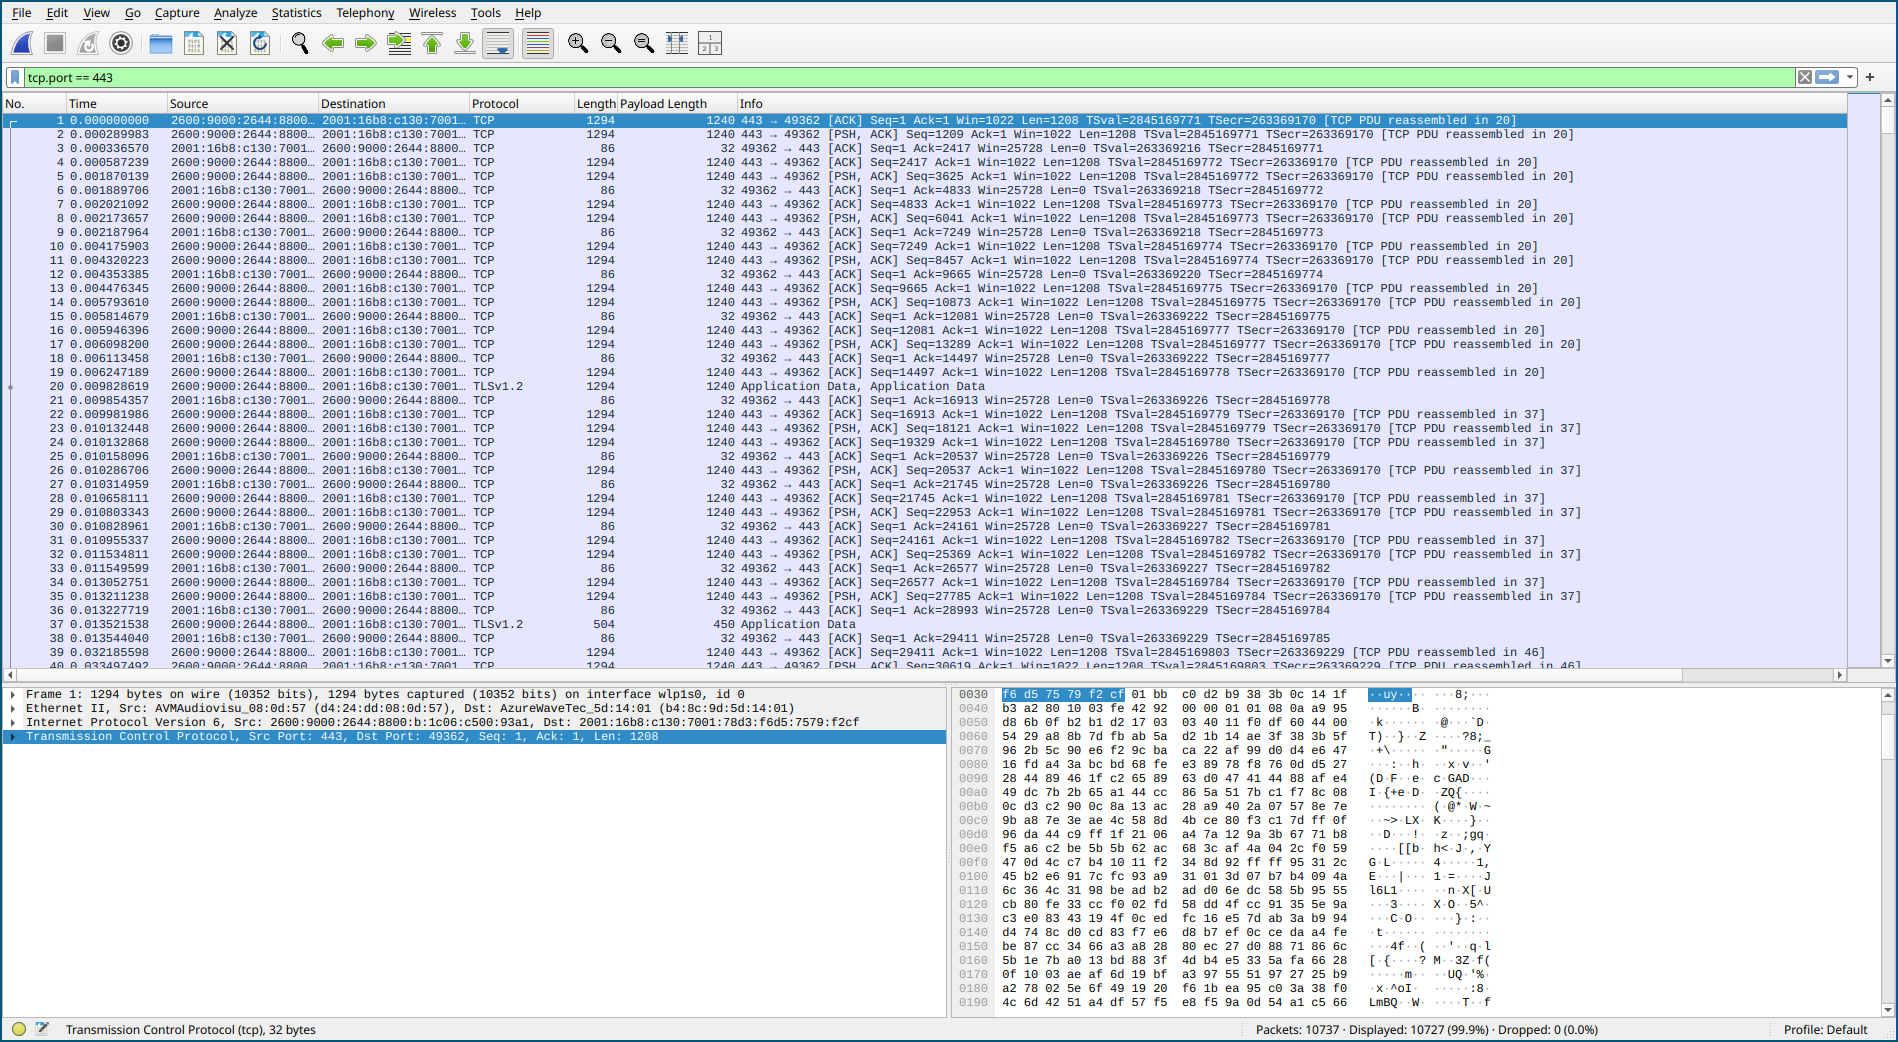
\includegraphics[width=1\textwidth]{./assets/5.1.a.https.png}
    \caption{HTTPS-Datenverkehr}
    \label{fig:5.1.a.https}
\end{figure}

\FloatBarrier

\begin{figure}[p]
    \centering
    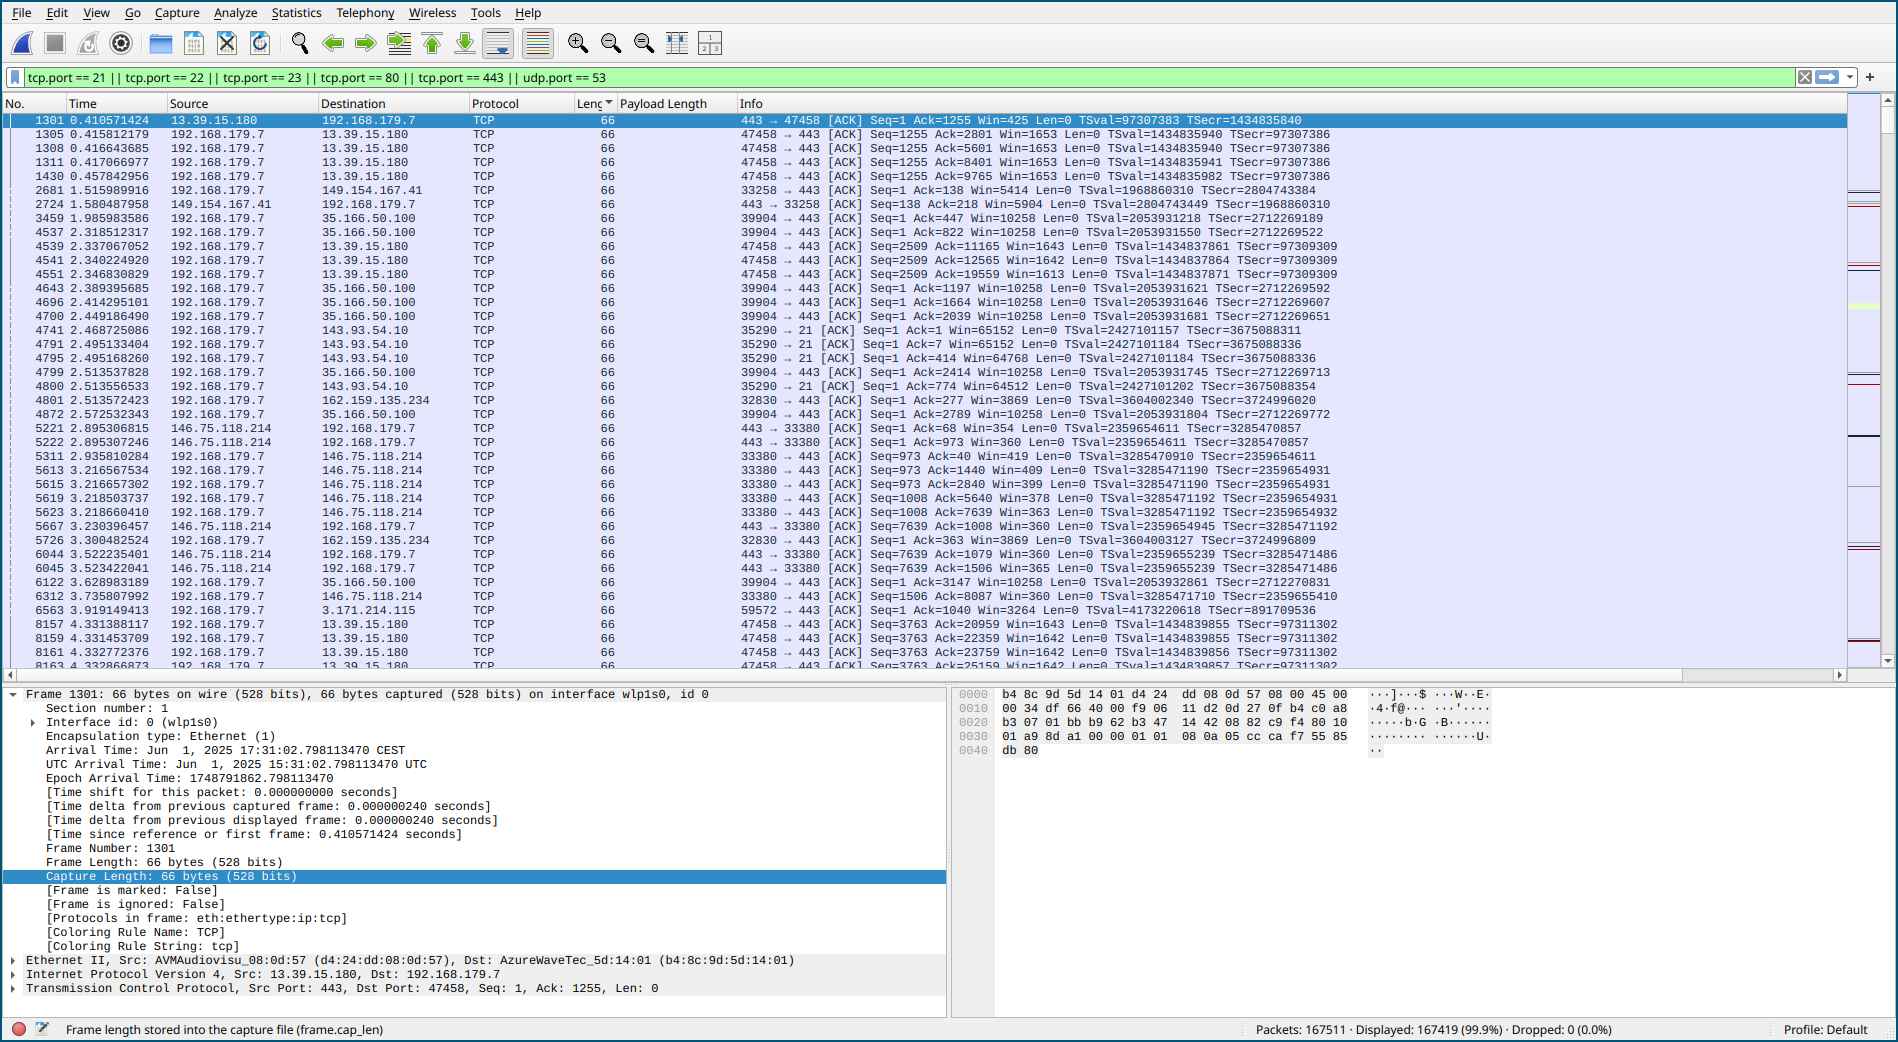
\includegraphics[width=1\textwidth]{./assets/5.1.b.1.png}
    \caption{kürzestes Segment}
    \label{fig:5.1.b.1}
\end{figure}

\begin{figure}[p]
    \centering
    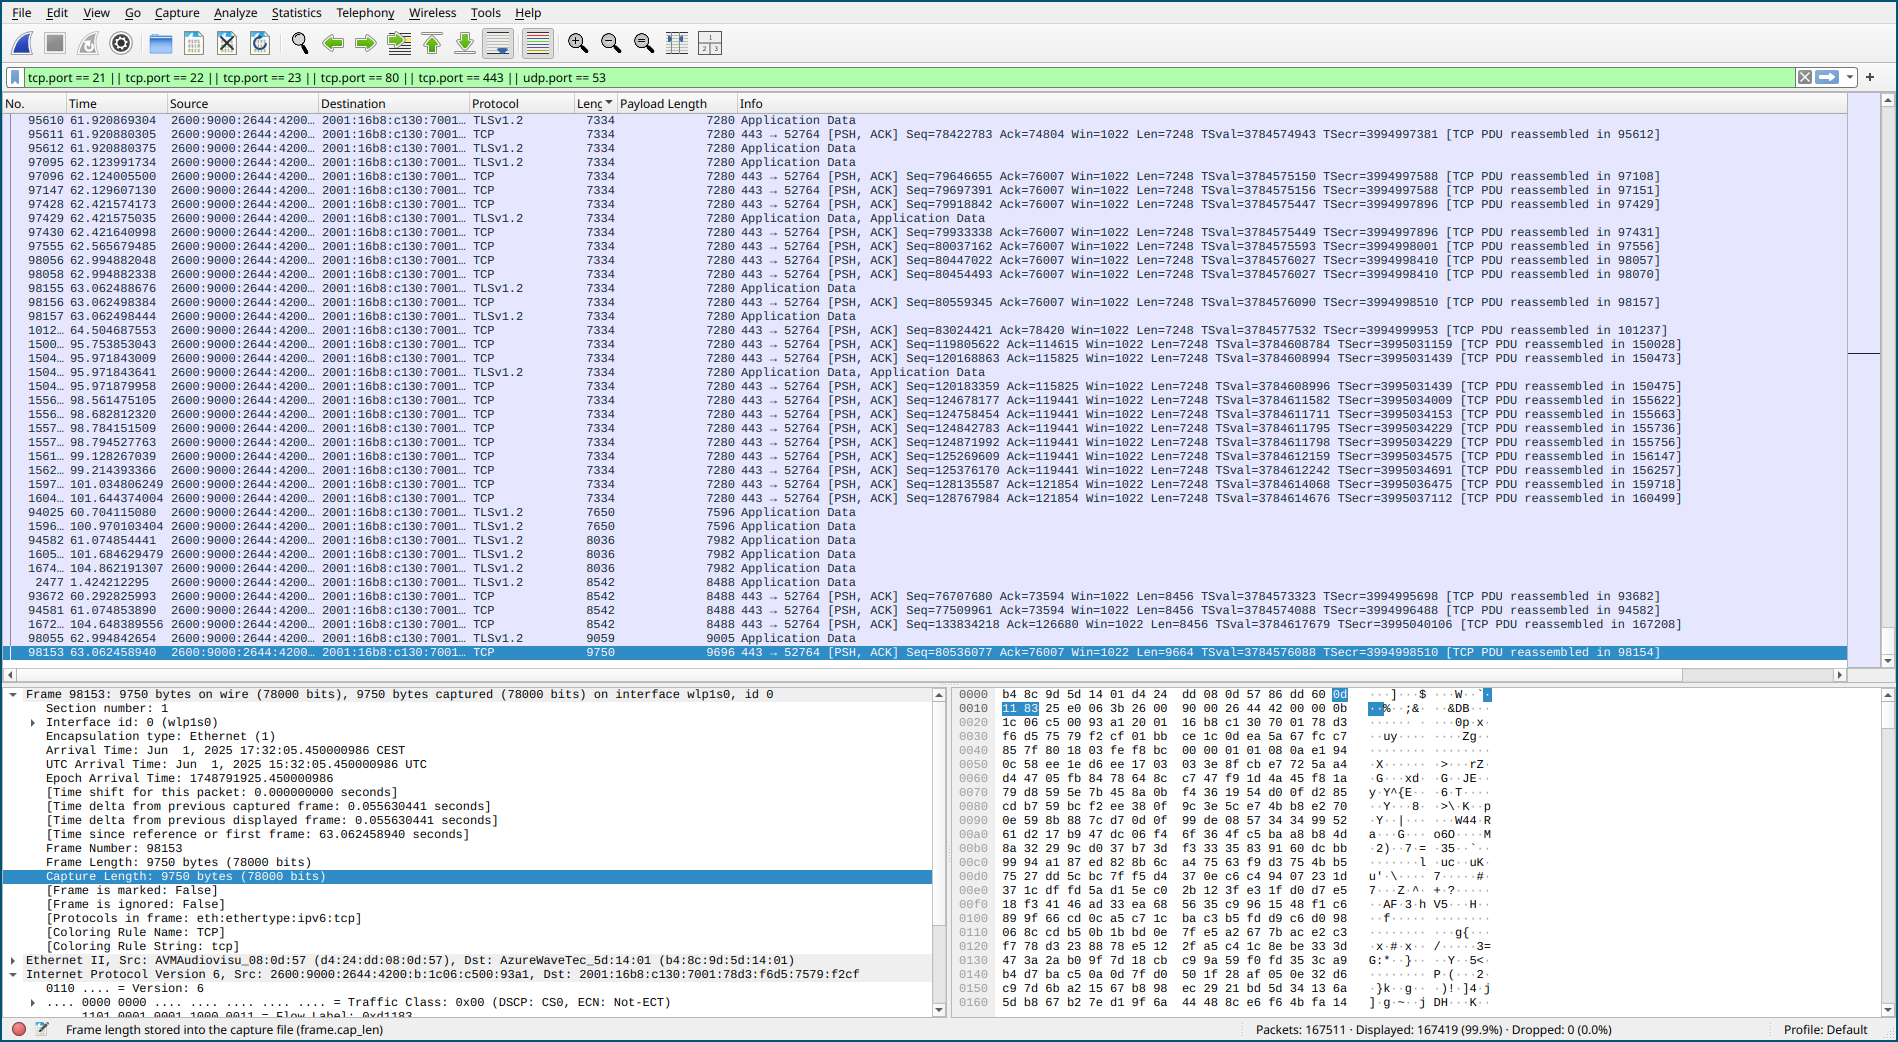
\includegraphics[width=1\textwidth]{./assets/5.1.b.2.png}
    \caption{längstes Segment}
    \label{fig:5.1.b.2}
\end{figure}

\FloatBarrier

\begin{figure}[p]
    \centering
    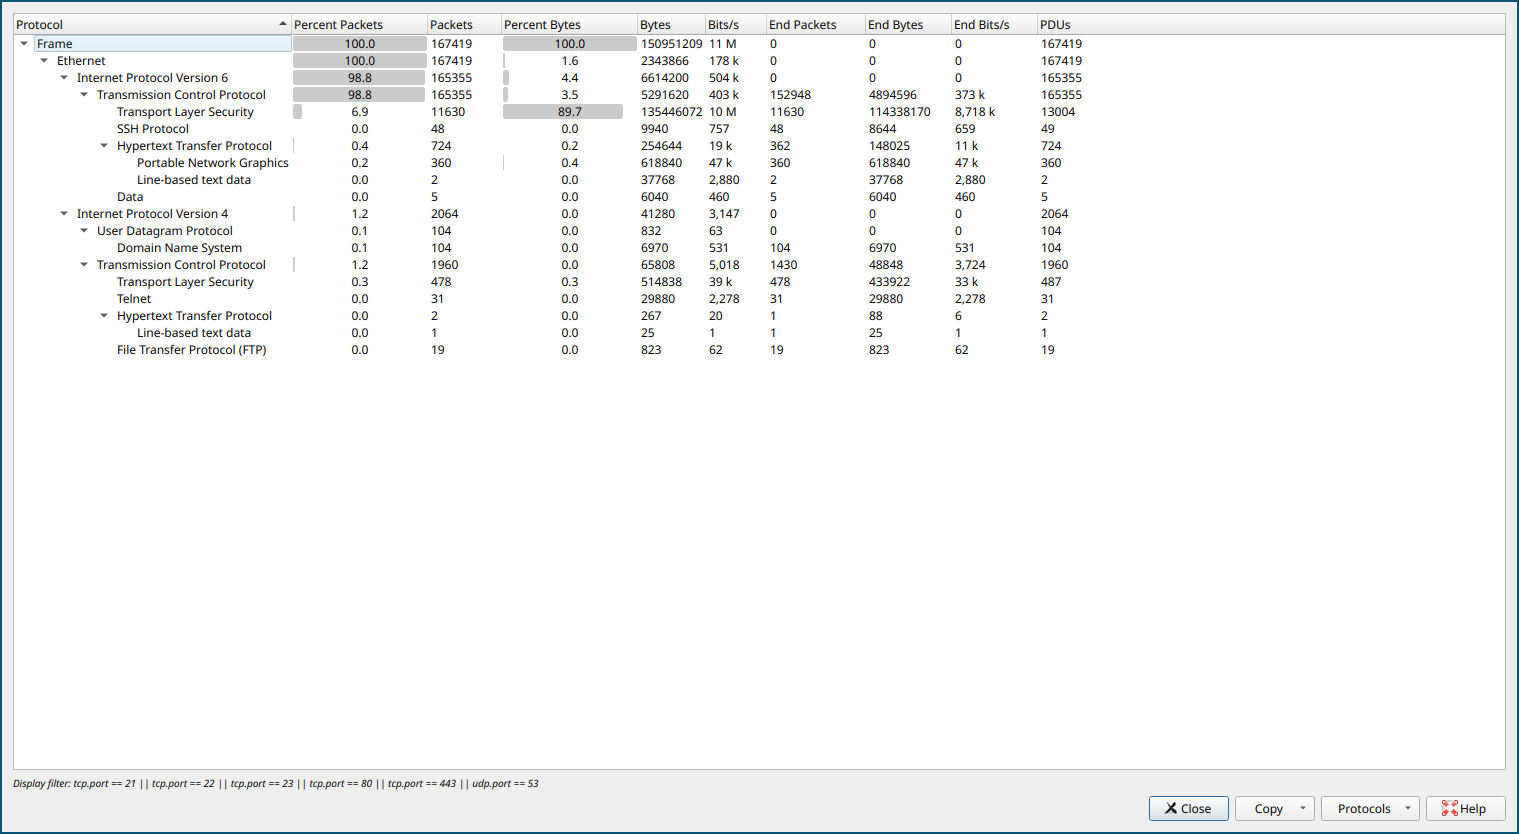
\includegraphics[width=1\textwidth]{./assets/5.1.c.png}
    \caption{Statistik aller verwendeten Anwendungsprotokolle}
    \label{fig:5.1.c}
\end{figure}

\FloatBarrier
